%------------------------------------------------------------------------------
% Author(s):
% Varaun Ramgoolie
% Copyright:
%  Copyright (C) 2020 Brad Bachu, Arjun Mohammed, Nicholas Sammy, Kerry Singh
%
%  This file is part of Applied-Mathematics-Unit2 and is distributed under the
%  terms of the MIT License. See the LICENSE file for details.
%
%  Description:
%     Year: 2012
%     Module: 1
%     Question: 1 
%------------------------------------------------------------------------------
\usetikzlibrary{patterns}

\begin{subquestions}

%------------------------------------------------------------------------------
% 1 a -------------------------------------------------------------------------
%------------------------------------------------------------------------------

\subquestion

Let $a$ be the number of backhoes of type $A$ and let $b$ be the number of backhoes of type $B$.

\begin{subsubquestions}
	
%------------------------------------------------------------------------------
% 1 a i------------------------------------------------------------------------
%------------------------------------------------------------------------------

\subsubquestion

The objective function that the contractor wants to maximize is,

\begin{equation}
	P = 40a + 60b \,.
\end{equation}

%------------------------------------------------------------------------------
% 1 a ii-----------------------------------------------------------------------
%------------------------------------------------------------------------------

\subsubquestion

The inequalities involved in this problem are,

\begin{align}
	a & \geq 0 \,, \nn \\
	b & \geq 0 \,, \nn \\
	50a + 20b & \leq 1000 \,, \nn \\
	2a + 8b & \leq 128\,, \nn \\
	a + b & \leq 25\,.
\end{align}

\end{subsubquestions}

%------------------------------------------------------------------------------
% 1 b--------------------------------------------------------------------------
%------------------------------------------------------------------------------

\subquestion

\begin{subsubquestions}

%------------------------------------------------------------------------------
% 1 b i------------------------------------------------------------------------
%------------------------------------------------------------------------------

\subsubquestion

See Graph ~\ref{2012:q1:graph:Graph1}.

\begin{figure}
	\centering
	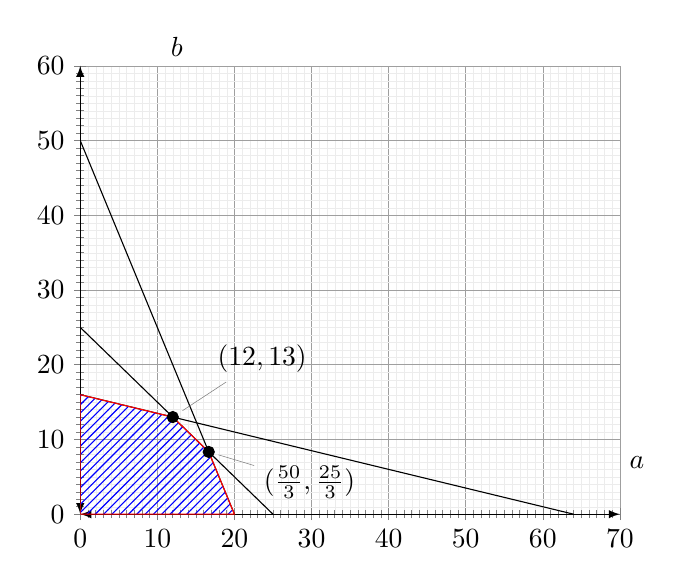
\begin{tikzpicture}
		\begin{axis}
			[
			xmin=-0,xmax=70,
			ymin=0,ymax=60,
			grid=both,
			grid style={line width=.1pt, draw=darkgray!10},
			major grid style={line width=.2pt,draw=darkgray!50},
			axis lines=left,
			minor tick num=9,
			enlargelimits={abs=0},
			axis line style={latex-latex},
			samples=100,
			domain = -20:20,
			ytick={0,10,...,60},
   			xlabel={$a$},
			ylabel={$b$},
			x label style={at={(axis description cs:1,0.15)},anchor=north west},
			y label style={at={(axis description cs:0.15,1)},anchor=south west, rotate=-90}
			]
			
			\addplot [mark=dot] coordinates{(25,0)  (0,25)};
			
			\addplot [mark=dot] coordinates {(64,0) (0,16)};
			
			\addplot [mark=dot] coordinates {(20,0) (0,50)};
			
			\addplot [red,pattern=north east lines,pattern color=blue] coordinates {(0,16) (12,13) (50/3, 25/3) (20,0)} \closedcycle;	
			
			\addplot [mark=*] coordinates{(12,13)};
		
			\node [pin=355:{$(\frac{50}{3},\frac{25}{3})$}] at (axis cs:50/3, 25/3) {};
			
			\addplot [mark=*] coordinates{(50/3, 25/3)};
			
			\node [pin=45:{$(12,13)$}] at (axis cs:12,13) {};
			
		\end{axis}
	\end{tikzpicture}
	\caption{\label{2012:q1:graph:Graph1} Graph showing the feasible region of the problem.} 
\end{figure}

%------------------------------------------------------------------------------
% 1 b ii------------------------------------------------------------------------
%------------------------------------------------------------------------------

\subsubquestion

The feasible region is shaded in Graph ~\ref{2012:q1:graph:Graph1}.

\end{subsubquestions}

%------------------------------------------------------------------------------
% 1 c------------------------------------------------------------------------
%------------------------------------------------------------------------------

\subquestion

\begin{subsubquestions}
	
%------------------------------------------------------------------------------
% 1 c i------------------------------------------------------------------------
%------------------------------------------------------------------------------

\subsubquestion

Using \rdef{mod1:defn:TourOfVertices},

\begin{align}
	\text{Using (0,16)} \,, \nn \\
	P & = 40a + 60b \,, \nn \\
	  & = (40 \times 0) + (60 \times 16) \,, \nn \\
	  & = 960 \,. \\
	\text{Using (20,0)} \,, \nn \\
	P & = 40a + 60b \,, \nn \\
      & = (40 \times 20) + (60 \times 0) \,, \nn \\
	  & = 800 \,. \\		  
	\text{Using (12,13)} \,, \nn \\
	P & = 40a + 60b \,, \nn \\
	  & = (40 \times 12) + (60 \times 13) \,, \nn \\
	  & = 1260 \,. \label{2012:q1:eqn:Profit} \\
	\text{Using ($\frac{50}{3}$, $\frac{25}{3}$)} \,, \nn \\
	P & = 40a + 60b \,, \nn \\
	  & = (40 \times \frac{50}{3}) + (60 \times \frac{25}{3}) \,, \nn \\
	  & = \frac{3500}{3} \approx 1166.67 \,. 
\end{align}

Thus, to maximize the amount of soil removed in 1 day, $12$ type A backhoes and $13$ type B backhoes should be used.

%------------------------------------------------------------------------------
% 1 c ii------------------------------------------------------------------------
%------------------------------------------------------------------------------

\subsubquestion

From \req{2012:q1:eqn:Profit}, the maximum weight that can be removed in 1 day is $1260$ tonnes.

\end{subsubquestions}

\end{subquestions}

